\documentclass[11pt,a4paper]{article}

\usepackage[T1]{fontenc}
\usepackage[utf8]{inputenc}
\usepackage{graphicx}
\usepackage{booktabs}
\usepackage{amsmath}
\usepackage{amssymb}
\usepackage{xcolor}
\usepackage{hyperref}
\usepackage{multirow}
\usepackage{array}
\usepackage{caption}
\usepackage{tikz}
\usepackage[margin=1in]{geometry}
\usetikzlibrary{arrows.meta, positioning, fit, shapes.geometric}

\hypersetup{colorlinks=true, linkcolor=blue, citecolor=blue, urlcolor=blue}

\title{CLeak: LLM-Orchestrated Unified Static and Dynamic Analysis\\
for C/C++ Memory Leak Detection}
\author{Dung Le Dang \\
\textit{Ho Chi Minh University of Information Technology}}
\date{}

\begin{document}

\maketitle

\begin{abstract}
Memory leaks (CWE-401) in C/C++ remain hard to find with either static or
dynamic analysis alone: static tools are noisy and cannot prove a leak
actually occurs at runtime, while dynamic tools only see the paths a test
run happens to exercise. Large language models (LLMs) can bridge this gap by
reading code and reasoning about ownership the way a human auditor would,
but naively giving an LLM a tool-calling loop over a codebase introduces the
opposite problem: non-deterministic, ungoverned, hard-to-reproduce
behavior that a scientific evaluation cannot rely on. We present
\textbf{CLeak}, a memory-leak investigation system for C/C++ that resolves
this tension with a single design principle: \emph{the LLM owns policy, the
deterministic engine owns mechanism}. Project-specific knowledge
(allocator/deallocator APIs, ownership conventions, analysis strategy,
judge calibration) is discovered once by an LLM, verified against source
text, frozen into a cached profile, and fed as parameters into a
deterministic static/dynamic engine that never consults the LLM on the
measured evaluation path. A four-stage HYBRID pipeline fans out static
sub-agents to gather evidence, runs a pinned build-and-sanitize dynamic
recipe in parallel, and reserves the LLM judge for genuinely borderline
verdicts, with a self-consistency \emph{consensus judge} fusing $K$
independent samples as the system's central judging contribution. A
two-tier reproducibility protocol reports bitwise-deterministic results for
the non-agentic configuration and honest mean$\pm$std / verdict-stability
statistics for the LLM-assisted configuration, rather than claiming
determinism the latter cannot have. On the full validated NIST Juliet
CWE-401 corpus (1{,}658 cases) the best end-to-end configuration reaches
Precision~77.9\%, Recall~77.3\%, F1~0.776, MCC~0.610. A controlled ablation
over five orchestration factors on a family-stratified sample ($n{=}100$)
isolates a deterministic static+dynamic+planner configuration that reaches
F1~0.932 at zero false positives, while showing that unconstrained
LLM-driven tool selection is $\sim$9$\times$ more expensive in tokens for no
accuracy gain. On seven real-world C projects from the peer-reviewed LAMeD
benchmark, the system achieves 100\% precision with recall rising from
0.159 to 0.273 as cross-function ownership evidence is added, including
one previously-unreported cJSON leak caught end-to-end. We report all of
this with explicit caveats where the evidence is incomplete or
inconclusive, in the interest of a reproducible and falsifiable
contribution.
\end{abstract}

\section{Introduction}
\label{sec:intro}

Missing release of memory after its effective lifetime, catalogued as
CWE-401, is one of the oldest and most persistent classes of software defects in C and
C++, the two languages in which manual memory management remains the norm
across operating-system kernels, browsers, databases, and embedded
firmware. Unlike a crash-inducing memory-safety bug (a buffer overflow or
use-after-free), a leak rarely terminates the process that causes it; it
manifests instead as slow resource exhaustion, degraded availability, or a
denial-of-service condition that is difficult to reproduce and expensive to
diagnose in production. The engineering cost of finding leaks has
historically been split between two incompatible tool families.
\textbf{Static analyzers} (Clang Static Analyzer, Facebook Infer, CodeQL)
reason about all paths through a program without executing it, which gives
them coverage but also a structurally high false-positive rate: without
running the program, a static tool cannot distinguish a genuine leak from
an allocation whose ownership was legitimately transferred to a caller.
\textbf{Dynamic analyzers} (Valgrind Memcheck, AddressSanitizer,
LeakSanitizer) instrument and run the actual binary, which gives them
near-zero false positives on the code paths they exercise, but zero
visibility into the (often much larger) set of paths a given test run does
not reach. Neither family alone is sufficient, and simple concatenation of
their findings does not resolve the disagreement between them.

Large language models offer a third analytical mode: reading a function's
source and its calling context and reasoning about ownership the way a
human code reviewer would, including project-specific conventions no
generic tool is aware of (a wrapper such as \texttt{cJSON\_Duplicate} is an
allocator; a parameter freed on the success path but not on an error path
is a leak on that path). The naive way to exploit this, giving an LLM
agent unrestricted tool access to a codebase and letting it decide what to
investigate, introduces exactly the property a controlled scientific
evaluation cannot tolerate: run-to-run non-determinism, even at
temperature~0, from provider-side batching and scheduling effects, together
with unconstrained and expensive tool-calling behavior that is hard to
audit or bound in cost.

CLeak's contribution is an architecture that captures the diagnostic value
of an LLM without inheriting its instability, organized around the design
principle stated in Section~\ref{sec:policy-mechanism}: \emph{the LLM owns
policy, the engine owns mechanism}. Concretely, this paper makes four
contributions:

\begin{description}
\item[C1: Consensus judge.] A judging layer that fuses static and
  dynamic evidence and, only for genuinely borderline bundles, resamples
  the LLM judge $K$ times at nonzero temperature and combines the votes by
  a self-consistency rule, materially reducing case-level verdict flip
  rate relative to a single LLM sample (Section~\ref{sec:judging}).
\item[C2: Two-tier reproducibility protocol.] A deterministic
  (\texttt{no\_llm}) configuration that is proven bitwise-reproducible by a
  dedicated determinism gate, and an LLM-assisted
  (\texttt{llm\_assisted}) configuration whose variance is measured and
  reported rather than hidden (Section~\ref{sec:reproducibility}).
\item[C3: Deterministic dynamic stage.] A pinned build-and-sanitize
  recipe that runs LeakSanitizer with zero LLM involvement whenever a
  project's build command is known, isolating dynamic evidence capture
  from LLM non-determinism (Section~\ref{sec:pipeline}).
\item[C4: Structured evidence enrichment.] Ownership-transfer tracking,
  alloc$\to$free pairing with guard-subset path reconciliation,
  path-sensitive and parameter-ownership leak detection, and
  runtime$\leftrightarrow$candidate correlation, that together make the
  purely deterministic heuristic judge path-aware without invoking an SMT
  solver (Section~\ref{sec:judging}).
\end{description}

We evaluate CLeak on the NIST Juliet CWE-401 suite (a validated,
integrity-checked 1{,}658-case subset), on the peer-reviewed LAMeD
real-world benchmark (41 developer-confirmed leaks across seven C
projects), and against live re-runs of Clang Static Analyzer and Infer on
identical scoring. Section~\ref{sec:evaluation} reports both the
full-corpus system result and a controlled five-factor ablation on a
family-stratified sample, explicitly labeled as answering two different
questions, together with a set of results we report as inconclusive or
partially superseded rather than omit.

\section{Related Work}
\label{sec:related}

\paragraph{Static analysis for memory leaks.}
Clang Static Analyzer~\cite{clangsa} and Facebook Infer~\cite{infer} use
path-sensitive symbolic execution over an intraprocedural or bounded
interprocedural scope, and CodeQL~\cite{codeql} expresses leak patterns as
queries over a database built from the program's AST/CFG/data-flow graph.
All three inherit the fundamental limitation of static reasoning about
memory: without a concrete execution, ownership transfer and conditional
deallocation are ambiguous, which drives false-positive rates up in
practice. Tree-sitter~\cite{treesitter} is not a leak detector but the
incremental-parsing substrate we and several of the systems below build on
for structural analysis. Neuro-symbolic hybrids such as
NESA~\cite{nesa} and general advances in scaling symbolic execution to
large codebases~\cite{symexec-scaling} point toward combining
learned and symbolic reasoning, a direction CLeak takes with an LLM instead
of a learned model.

\paragraph{Dynamic analysis for memory leaks.}
Valgrind Memcheck~\cite{valgrind} and
AddressSanitizer / LeakSanitizer~\cite{asan} instrument and run a binary
directly, giving near-perfect precision on exercised paths at the cost of
path coverage. Recent sanitizer research (RangeSanitizer~\cite{rangesan},
QMSan~\cite{qmsan}, CombiSan~\cite{combisan}, and taint-analysis
accelerators such as AirTaint~\cite{airtaint}) improves detection speed and
precision for related memory-safety classes but does not address dynamic
analysis's coverage ceiling. A direct empirical comparison of fuzzers
against static analyzers for memory-unsafety detection~\cite{fuzzer-vs-sa}
finds the two tool families' true-positive sets are largely disjoint ---
motivating the hybrid design in Section~\ref{sec:pipeline} rather than a
choice between them. AddressWatcher~\cite{addresswatcher} localizes leak
\emph{fixes} from sanitizer output, a complementary problem to detection.

\paragraph{LLMs for software defect detection.}
Early empirical work established that LLMs can identify security
vulnerabilities from source alone with meaningful but bounded
accuracy~\cite{llm-vuln-eval}. IRIS~\cite{iris} couples an LLM with static
analysis for vulnerability detection; a complementary line of work asks
whether LLM prompting alone can substitute for a static analyzer's
reasoning~\cite{llm-proxy-static}, generally finding it cannot without
tool grounding. VulnLLM-R~\cite{vulnllmr} and SemTaint~\cite{semtaint}
represent, respectively, a reasoning-specialized model and a multi-agent
taint-specification extractor for vulnerability classes broader than
leaks. Two systems target C/C++ memory leaks directly and are the closest
prior work to CLeak: \textbf{MemHint}~\cite{memhint}, a
neuro-symbolic-augmented static pipeline (LLM + Z3 + CodeQL/Infer) reporting
52--54 confirmed leaks across real projects, and
\textbf{LAMeD}~\cite{lamed}, which uses an LLM purely to \emph{annotate}
source for a classical analyzer (Cooddy or CodeQL) to then consume ---
notably \emph{not} an agentic architecture, and the origin of the
real-world benchmark we evaluate against in
Section~\ref{sec:eval-lamed}. LAMeD does not report an F1 score; we quote
its own published precision/recall where we compare against it.
A related but distinct line targets kernel-level memory-management
intention inconsistencies~\cite{kernel-memmgmt}.
Agentic multi-agent systems for repository-scale auditing, including
RepoAudit~\cite{repoaudit}, Revelio~\cite{revelio}, SAILOR~\cite{sailor},
and crash-oriented systems such as FuzzingBrain~V2~\cite{fuzzingbrainv2}
and ATLANTIS~\cite{atlantis} (an AIxCC Cyber Reasoning System), are
architectural analogues we draw on for agent design, but target
multi-defect classes (use-after-free, null-pointer dereference, or
crash-reproducing exploits generally) rather than non-crash leaks
specifically, and RepoAudit's own reported P=78.4\% spans several defect
types, not leaks alone, so we do not treat it as a leak-specific baseline.
Foundational agent-design work, including ReAct~\cite{react},
Reflexion~\cite{reflexion}, Tree-of-Thoughts~\cite{tot}, and the
SE-specific agent scaffolds SWE-agent~\cite{sweagent} and
Agentless~\cite{agentless}, informs the hard tool-partitioning and
completion-nudge mechanisms of our Stage~A/B sub-agents
(Section~\ref{sec:pipeline}).

\paragraph{Reducing LLM variance and LLM-as-judge.}
Self-consistency decoding~\cite{selfconsistency}, which samples multiple
reasoning chains at nonzero temperature and aggregates them by vote, is the
mechanism our consensus judge (C1) applies to leak verdicts rather than
chain-of-thought answers. Zheng et al.'s study of LLM-as-a-judge
calibration and disagreement~\cite{llmjudge} motivates why we treat a
single LLM sample as insufficiently stable to trust unconditionally and
report McNemar-test significance (Section~\ref{sec:eval-consensus}) rather
than a raw accuracy delta.

\paragraph{Benchmarks and protocols.}
We use the NIST Juliet Test Suite~\cite{juliet} as our synthetic
ground-truth corpus and the LAMeD benchmark~\cite{lamed-benchmark} as our
real-world, peer-reviewed corpus; DiverseVul~\cite{diversevul},
SV-COMP Memsafety~\cite{svcomp}, and Magma~\cite{magma} are related
vulnerability/memory-safety benchmarks we do not use directly but position
against in corpus design. The Model Context Protocol~\cite{mcp} is the
tool-invocation transport between our orchestrator and analyzers
(Section~\ref{sec:arch}); a pointer-ownership model for
C~\cite{ownership-model} informs the ownership-transfer vocabulary used by
our heuristic judge.

\paragraph{Positioning.} To our knowledge, no system in the 2025--2026
literature combines static and dynamic evidence specifically for
\emph{non-crash} C/C++ memory leaks while also providing a reproducibility
protocol distinguishing deterministic from LLM-dependent results. CLeak is
designed to fill exactly this gap. Table~\ref{tab:capability} makes this
comparison explicit across eleven capability criteria drawn from the
systems discussed above; no single prior system combines static analysis,
dynamic analysis, agentic orchestration, and a verified bit-for-bit
reproducibility gate the way CLeak does, and CLeak is, to our knowledge,
the only one of the seven that both exposes an MCP tool transport and
generates a source-anchored repair diff alongside its verdicts.

\begin{table}[htbp]
\centering
\caption{Core capability matrix. \checkmark{} = yes, $\times$ = no,
$\circ$ = partial / conditional, $\bullet$ = present but secondary (not
the system's focus), --- = not applicable or unpublished. The
\emph{deterministic core} row is distinct from \emph{bit-for-bit
reproducibility}: LAMeD's Cooddy backend is itself deterministic but its
version is not pinned; MemHint and POM have a deterministic
symbolic/SAT core but a non-deterministic LLM labeling step precedes it;
RepoAudit and FuzzingBrain~V2 are end-to-end agentic pipelines with no
deterministic tier at all. CLeak is the only system in this comparison
verified, by a dedicated gate, to reproduce byte-identical scoring across
independent runs (Section~\ref{sec:reproducibility}).}
\label{tab:capability}
\resizebox{\textwidth}{!}{%
\begin{tabular}{@{}lccccccc@{}}
\toprule
\textbf{Criterion} & \textbf{LAMeD} & \textbf{MemHint} & \textbf{RepoAudit} & \textbf{FuzzingBrain V2} & \textbf{POM} & \textbf{SecVulEval} & \textbf{CLeak} \\
\midrule
LLM involved & \checkmark & \checkmark & \checkmark & \checkmark & \checkmark & --- & \checkmark \\
MCP tool transport & $\times$ & $\times$ & $\times$ & \checkmark & $\times$ & --- & \checkmark \\
Static analysis & \checkmark & \checkmark & $\circ$ & \checkmark & \checkmark & --- & \checkmark \\
Dynamic analysis (sanitizer/Valgrind) & $\times$ & $\times$ & $\times$ & \checkmark & $\times$ & --- & \checkmark \\
Deterministic core (no LLM in decision path) & \checkmark & \checkmark & \checkmark & $\circ$ & \checkmark & --- & \checkmark \\
\textbf{Bit-for-bit reproducibility (gate-verified)} & $\times$ & $\times$ & $\times$ & $\times$ & $\times$ & --- & \textbf{\checkmark} \\
Memory-leak (C/C++) specialized & \checkmark & \checkmark & $\circ$ & $\bullet$ & $\bullet$ & $\times$ & \checkmark \\
Agentic orchestration & $\times$ & $\times$ & \checkmark & \checkmark & $\times$ & --- & \checkmark \\
Judge / validator layer & $\circ$ & \checkmark & \checkmark & $\circ$ & \checkmark & --- & \checkmark \\
Repair-diff generation & $\times$ & $\times$ & $\times$ & $\times$ & $\times$ & --- & \checkmark \\
Peer-reviewed & \checkmark (EASE'25) & $\times$ (arXiv) & $\circ$ (poster) & $\times$ (arXiv) & $\times$ (tech rep.) & $\times$ (withdrawn) & --- (this work) \\
\bottomrule
\end{tabular}}
\end{table}

\section{System Architecture}
\label{sec:arch}

\subsection{Component overview}

CLeak is a standalone CLI/TUI scanner, \texttt{leak-inspector-tui}, acting
as the sole orchestrator; it drives two analyzer services and an LLM
provider over well-defined protocols, with no shared database and no
persistent server-side state beyond per-run artifacts on disk. All
inter-service communication uses the Model Context Protocol (MCP) over
Streamable-HTTP (JSON-RPC~2.0). Table~\ref{tab:components} summarizes
the four components; Figure~\ref{fig:topology} shows their connectivity.

\begin{table}[htbp]
\centering
\caption{System components.}
\label{tab:components}
\small
\begin{tabular}{@{}p{2.6cm}p{3.6cm}p{1.2cm}p{6.6cm}@{}}
\toprule
\textbf{Component} & \textbf{Technology} & \textbf{Port} & \textbf{Responsibility} \\
\midrule
leak-inspector-tui & TypeScript + Ink (Node), native tool-calling & headless & Orchestrator: MCP client, agentic loop, report writer \\
static-analyzer & NestJS + tree-sitter & 50061 & 11 MCP tools: candidate scan, AST/call-graph, function summary, path constraints, ownership, Clang \texttt{scan-build} \\
dynamic-analyzer & NestJS + Valgrind/ASan/LSan & 50062 & 11 MCP tools: sanitizer build/run, targeted-harness synthesis (opt-in) \\
agent-core / common (libraries) & TypeScript & --- & Tool-calling loop, MCP client, multi-provider LLM adapters; shared types, heuristic/consensus judge, report renderers \\
\bottomrule
\end{tabular}
\end{table}

\begin{figure}[htbp]
\centering
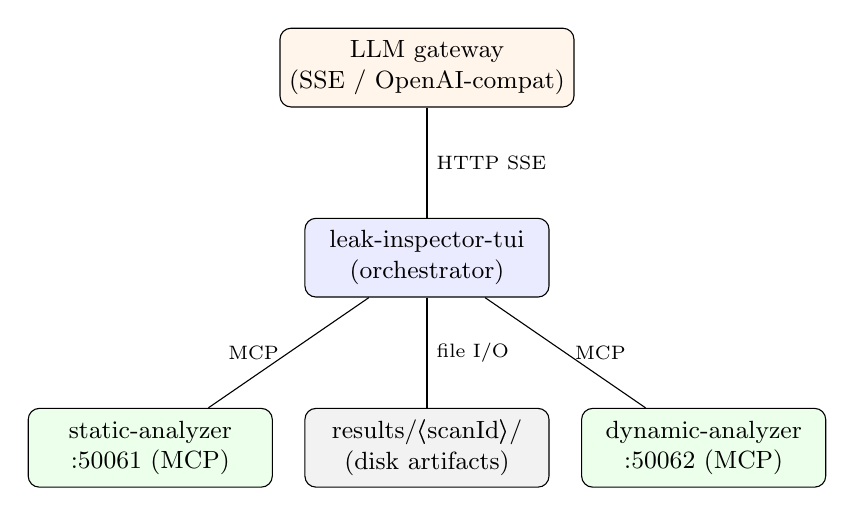
\begin{tikzpicture}[
  node distance=1.1cm and 1.6cm,
  box/.style={draw, rounded corners, minimum width=3.1cm, minimum height=1cm, align=center, font=\small},
  every edge/.style={draw, -Stealth, thick}
]
  \node[box, fill=blue!8] (tui) {leak-inspector-tui\\(orchestrator)};
  \node[box, below left=1.4cm and 0.4cm of tui, fill=green!8] (static) {static-analyzer\\:50061 (MCP)};
  \node[box, below right=1.4cm and 0.4cm of tui, fill=green!8] (dynamic) {dynamic-analyzer\\:50062 (MCP)};
  \node[box, above=1.4cm of tui, fill=orange!8] (llm) {LLM gateway\\(SSE / OpenAI-compat)};
  \node[box, below=1.4cm of tui, fill=gray!10] (results) {results/\textlangle scanId\textrangle/\\(disk artifacts)};

  \draw (tui) -- node[left, font=\scriptsize] {MCP} (static);
  \draw (tui) -- node[right, font=\scriptsize] {MCP} (dynamic);
  \draw (tui) -- node[right, font=\scriptsize] {HTTP SSE} (llm);
  \draw (tui) -- node[right, font=\scriptsize] {file I/O} (results);
\end{tikzpicture}
\caption{System topology. The orchestrator is the sole client of both
analyzer services and the LLM gateway; the two analyzers never communicate
directly with each other or with the LLM.}
\label{fig:topology}
\end{figure}

\subsection{Policy versus mechanism}
\label{sec:policy-mechanism}

The architecture's organizing principle is that \emph{the LLM owns
policy, the engine owns mechanism}. Anything that varies per project
(which functions allocate memory, what the project's ownership conventions
are, how aggressively to run dynamic analysis, how to calibrate verdict
thresholds) is discovered once by an LLM, exported as a structured
profile, \emph{verified} against the source text it was derived from (a
grep-based anti-hallucination check), cached to disk, and then frozen for
benchmarking. The engine itself (tree-sitter parsing, control-flow
construction, alloc$\to$free pairing, heuristic scoring, and consensus
aggregation) executes deterministically and never depends on the LLM on
the measured evaluation path. Three host-side modules implement this
pattern (Table~\ref{tab:policy}); onboarding a new project therefore
requires zero lines of new code.

\begin{table}[htbp]
\centering
\caption{The three POLICY modules and what they decide.}
\label{tab:policy}
\small
\resizebox{\textwidth}{!}{%
\begin{tabular}{@{}p{2.6cm}p{5.4cm}p{2.8cm}p{3.6cm}@{}}
\toprule
\textbf{Module} & \textbf{LLM decides} & \textbf{Verification} & \textbf{Feeds into} \\
\midrule
Allocator profiler & Project alloc/dealloc API names + ownership notes & Identifier must literally appear in source (grep) & \texttt{extraAllocators} / \texttt{Deallocators}, ownership notes \\
Strategist & \{runDynamic, judge mode, staticDepth\} & Rule-based deterministic fallback on failure & Gates the dynamic stage / fan-out \\
Judge tuner & Verdict-threshold nudge & Hard clamp to a bounded range & Heuristic judge thresholds (production only; eval uses frozen defaults) \\
\bottomrule
\end{tabular}}
\end{table}

In the benchmark configuration used throughout Section~\ref{sec:evaluation},
allocators are supplied from a frozen manifest and the strategist/tuner are
disabled, so there are \emph{zero} non-deterministic LLM calls on the
evaluation path for the \texttt{no\_llm} mode, and the Juliet baseline
confusion matrix (TP29/FP7/FN3 at $n{=}30$) is fixed across runs.

\subsection{Data model}

Findings from every analysis tool converge on a common structure:
a \texttt{LeakCandidate} (an allocation site) accumulates \texttt{Evidence}
entries (Valgrind/ASan/LSan/\texttt{scan-build}/heuristic) into a
\texttt{LeakBundle}, which the judging layer (Section~\ref{sec:judging})
resolves into a \texttt{VerdictResult}: a verdict label, a confidence
score, a natural-language explanation, a root cause, and a source-anchored
repair diff. Verdicts are written by code, never by free-form LLM text: an
LLM can only cause a verdict change through the two well-defined
interfaces of Sections~\ref{sec:judging}. All artifacts for a run
(\texttt{report.json/md/html}, a cross-run-comparable
\texttt{snapshot.json}, an append-only event log, and a metrics summary)
are written to \texttt{results/\textlangle scanId\textrangle/} on disk; there is no
database.

\subsection{MCP tool surface}

The static and dynamic analyzers together expose 22 MCP tools, but only
five are given directly to the LLM sub-agent of Stage~A
(Section~\ref{sec:pipeline}): \texttt{candidateScan}, \texttt{astScan},
\texttt{functionSummary}, \texttt{pathConstraints}, and
\texttt{ownershipConventions}. These are the \emph{content-capable} tools
--- they accept inline source content rather than requiring a shared
filesystem mount, which keeps both analyzer services stateless and
independently deployable. The remaining tools (indexing,
call-graph/interprocedural-flow extraction, \texttt{scan-build}
orchestration, and all dynamic build/sanitizer tools) are driven directly
by the orchestrator, not by the LLM, because they either require
filesystem access the analyzer does not have or are part of the
deterministic Stage~B recipe described next.

\section{The HYBRID Investigation Pipeline}
\label{sec:pipeline}

Once static candidates are discovered (a deterministic
\texttt{candidateScan} over allocation sites, using the project's frozen
allocator profile), each candidate is bundled and investigated through
four stages, shown in Figure~\ref{fig:pipeline}.

\begin{figure}[htbp]
\centering
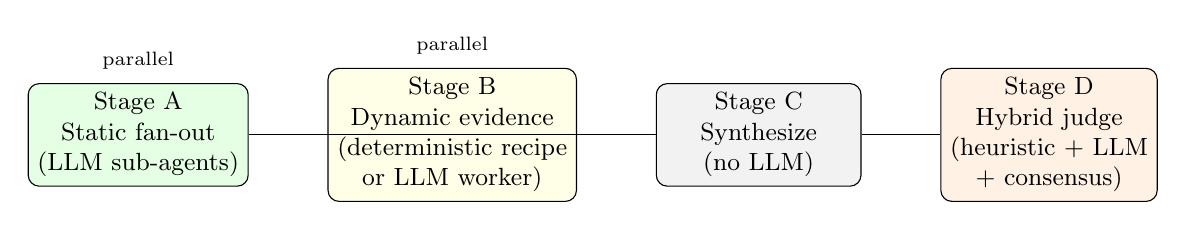
\begin{tikzpicture}[
  node distance=0.55cm and 1.0cm,
  stg/.style={draw, rounded corners, minimum width=2.6cm, minimum height=1.05cm, align=center, font=\small},
  every edge/.style={draw, -Stealth, thick}
]
  \node[stg, fill=green!10] (a) {Stage A\\Static fan-out\\(LLM sub-agents)};
  \node[stg, right=of a, fill=yellow!10] (b) {Stage B\\Dynamic evidence\\(deterministic recipe\\or LLM worker)};
  \node[stg, right=of b, fill=gray!10] (c) {Stage C\\Synthesize\\(no LLM)};
  \node[stg, right=of c, fill=orange!10] (d) {Stage D\\Hybrid judge\\(heuristic + LLM\\+ consensus)};
  \draw (a) -- (c);
  \draw (b) -- (c);
  \draw (c) -- (d);
  \node[font=\scriptsize, above=0.05cm of a] {parallel};
  \node[font=\scriptsize, above=0.05cm of b] {parallel};
\end{tikzpicture}
\caption{The four-stage HYBRID pipeline. Stages A and B run concurrently
over the same candidate bundles; Stage C performs no LLM reasoning; Stage
D escalates to the LLM only for borderline bundles (Section~\ref{sec:judging}).}
\label{fig:pipeline}
\end{figure}

\textbf{Stage A: static fan-out.} Candidates are grouped by file
affinity into small batches, each assigned to an independent LLM sub-agent
restricted to the five content-capable static tools of
Section~\ref{sec:arch} plus a \texttt{read\_file} tool. The sub-agent
gathers structural evidence (ownership conventions, path constraints,
function-level alloc/free pairing) but is explicitly instructed, and
architecturally unable by tool partitioning, to record a verdict.
Evidence is captured automatically by code wrapping each tool call, not
self-reported by the model, which removes one common source of agent
hallucination from the evaluation path.

\textbf{Stage B: dynamic evidence.} Whenever the case carries a known
build command (as Juliet cases do, by NIST's own convention), Stage~B runs
a \emph{fixed, deterministic} recipe: \texttt{buildTarget} with
sanitizer flags followed by \texttt{lsanRun}, with no LLM call
whatsoever (contribution C3). This is what makes the \texttt{no\_llm}
configuration's dynamic evidence reproducible bit-for-bit. Only when no
build command is known does control fall back to an LLM dynamic worker
that reads the project's build system and attempts its own sanitizer
build; this worker is restricted to the nine dynamic tools plus
\texttt{read\_file} and runs concurrently with Stage~A.

\textbf{Stage C: synthesis.} A purely deterministic merge of static
context and dynamic evidence into each bundle, stamping a
\texttt{dynamicCoverage} state (\texttt{exercised\_clean},
\texttt{exercised\_leak}, \texttt{not\_exercised}, or \texttt{dynamic\_off})
that the judging layer treats as ground truth about what was actually
observed at runtime. No LLM call occurs in this stage.

\textbf{Stage D: hybrid judging} is described in full in
Section~\ref{sec:judging}. Any model-call or parse failure at any stage
falls back to the deterministic heuristic verdict, so the system is
architecturally biased toward being no worse than its deterministic core,
never toward silent failure.

\section{Judging Layer}
\label{sec:judging}

CLeak's judging layer has three interchangeable configurations, evaluated
head-to-head throughout Section~\ref{sec:evaluation}: a purely
\textbf{heuristic judge}, a \textbf{single-LLM judge}, and a
\textbf{consensus judge}. The heuristic judge always runs first and scores
every bundle; only bundles it leaves \emph{borderline} are escalated.

\subsection{Heuristic judge: deterministic, path-sensitive}

The heuristic judge (contribution C4) sums a fixed table of weighted
evidence signals per bundle: correlated runtime leaks (weighted by
sanitizer leak kind: \texttt{definitely\_lost}/\texttt{asan\_leak} weigh
most, \texttt{possibly\_lost} least), structural missing-free patterns,
unpaired or conditionally-freed allocations, a \emph{path-sensitive leak}
signal, a \emph{parameter-ownership leak} signal, and an
ownership-transfer penalty when the allocation is legitimately handed to a
caller. It then bands the total score against fixed thresholds,
$\mathit{confirmed}=0.7$ and $\mathit{likely}=0.4$, frozen for every
evaluation run reported in this paper. Three precision gates can override
the additive score outright: a callee-freed allocation with no correlated
runtime leak is forced to \texttt{likely\_false\_positive}; a clean dynamic
run with no decisive static evidence exculpates a candidate; and any
``flagged'' verdict lacking at least one \emph{strong} signal (a correlated
runtime leak, a high-confidence structural pattern, an unpaired
allocation, a path-sensitive leak, or an ownership issue) is downgraded to
\texttt{uncertain} rather than reported as a leak.

\textbf{Path sensitivity without an SMT solver.} CLeak computes path
feasibility with a lightweight heuristic rather than an SMT solver, so
guard analysis is unconditionally available on every function it analyzes
with no solver-timeout or memory-ceiling failure mode. This mechanism,
\emph{guard-subset reconciliation}, works as follows: a free on one control-flow path
reconciles an allocation only if that free's guard condition set is a
\emph{subset} of the exit path's guard set: a free reachable under
a strictly narrower condition than the corresponding leak exit does not
count as covering it. This heuristic CFG analysis, combined with
conservative dead-code reachability (dropping exit paths that follow an
unconditional terminator in the same block), is what lets even the
deterministic \texttt{no\_llm} judge catch leaks such as a pointer freed on
a function's success path but lost on its error path (a
\emph{path-sensitive leak}) or a parameter freed on some branches but not
others (a \emph{parameter-ownership leak}). This is the exact pattern behind
cJSON's \texttt{merge\_patch} case study in
Section~\ref{sec:eval-lamed}.

\subsection{LLM judge: rubric-based, borderline-only}

A bundle escalates to the LLM judge when the heuristic verdict is
\emph{borderline} (\texttt{likely\_leak} or \texttt{uncertain}, or
confidence in $[0.35, 0.7]$) \emph{or} there is an explicit contradiction
between the heuristic verdict and dynamic evidence (e.g.\ flagged as a leak
but a correlated sanitizer run came back clean). The LLM sees the
candidate's enclosing function source (labels stripped from any comments
to avoid leaking benchmark ground truth), a summary of static evidence,
dynamic findings tagged by correlation strength
(\texttt{LINKED} / same-file-different-site / \texttt{CLEAN}), and, when
available, the project's LLM-discovered ownership conventions. It returns
one of five labels with a confidence and an explanation, following an
explicit priority rubric: a linked runtime leak is decisive; ownership
transfer is decisive for false positives; the same path-sensitive and
parameter-ownership rules used by the heuristic judge apply; and
\texttt{uncertain} is reserved for genuinely insufficient evidence, not a
default. No native tool-calling is exposed at this stage (output is
constrained to JSON); a parse failure of any kind silently falls back to
the heuristic verdict.

\subsection{Consensus judge: self-consistency voting (C1)}

When enabled ($K>1$), the same LLM-judge call is resampled $K$ times at a
nonzero consensus temperature and the results merged by one of three rules:
majority, a confidence-weighted vote (with dynamic-contradicting votes
down-weighted $\times 0.3$), or unanimous-to-flag, with the final label
taken as the modal verdict within the flagging cluster. A veto rule
ensures asymmetry: a strong heuristic exculpation (a
\texttt{false\_positive}/\texttt{likely\_false\_positive} verdict at
confidence $\geq 0.75$) can only \emph{remove} a flag from the consensus
outcome, never add one. Consensus voting is designed to reduce false
positives introduced by a single unstable LLM sample, not to introduce new
ones. Section~\ref{sec:eval-consensus} evaluates the effect of this
mechanism directly.

\section{Reproducibility Protocol}
\label{sec:reproducibility}

An LLM-in-the-loop system cannot honestly claim bit-identical
reproducibility, and we do not: CLeak instead reports a
\textbf{two-tier} protocol (contribution C2) that distinguishes what is
and is not deterministic.

\textbf{Tier 1: \texttt{no\_llm}, bitwise-deterministic.} With the
strategist/tuner disabled and allocators supplied from a frozen manifest,
the heuristic judge, the deterministic Stage~B recipe, and the scoring
pipeline together produce byte-identical output across runs. This is
enforced, not merely claimed: a dedicated determinism gate runs the same
configuration twice into distinct output directories and asserts an
identical confusion matrix, per-variant metrics, per-case rows, and
judge-path distribution. During development, the gate caught and now
explicitly rejects two \emph{false-pass} modes: a coarse-grained timestamp
collision that caused the tool to compare a run against itself, and a
degenerate run in which an unreachable analyzer made every case error out
\emph{identically}, which would otherwise register as spurious
determinism.

\textbf{Tier 2: \texttt{llm\_assisted}, reported variance.} Because
even temperature-0 LLM calls are not bit-identical across runs (provider
batching, floating-point non-associativity, and scheduling effects), we
run each \texttt{llm\_assisted} configuration $N$ times and report
mean$\pm$std for every metric, together with a \emph{case-level
verdict-stability} analysis: the percentage of cases whose verdict does
not change across runs, the flip rate, and modal agreement. We surface an
explicit \textbf{stable-by-luck} phenomenon we observed directly: two
independent 30-case runs produced an \emph{identical} aggregate confusion
matrix (27~TP/8~FP/5~FN/37~TN) while only 73.3\% of individual case
verdicts were actually stable (a 26.7\% flip rate); flips in opposite
directions cancelled out in the aggregate. Reporting only the aggregate
matrix would have concealed this; reporting case-level stability does not.

\section{Evaluation}
\label{sec:evaluation}

\subsection{Experimental setup}

\textbf{Datasets.} Table~\ref{tab:datasets} summarizes the three corpora.
The Juliet corpus is passed through a five-gate integrity pipeline (Zod
schema validation, \texttt{\#include} resolution, per-translation-unit
\texttt{clang -fsyntax-only}, label-overlap checking, and a content-hash
lock) before any evaluation run is permitted against it; an earlier,
unvalidated ingest had silently dropped 21\% of C++ multi-file class
variants from the confusion matrix, and all headline numbers in this
paper are measured on the corrected, validated 1{,}658-case corpus. LAMeD
is \emph{positive-only} at the function level (no line numbers, no
negative/clean labels), so true negatives are zero by construction; we
therefore report only recall, precision, and false positives per KLOC for
it, never specificity, accuracy, or MCC.

\begin{table}[htbp]
\centering
\caption{Evaluation corpora.}
\label{tab:datasets}
\small
\begin{tabular}{@{}p{2.6cm}p{2.4cm}p{2.6cm}p{5.4cm}@{}}
\toprule
\textbf{Corpus} & \textbf{Size} & \textbf{Type} & \textbf{Notes} \\
\midrule
Juliet CWE-401~\cite{juliet} & 1{,}658 validated cases (10 functional families) & Synthetic, function-labeled & NIST SARD; validated by a 5-gate integrity pipeline + lockfile \\
LAMeD~\cite{lamed-benchmark} & 41 leaks / 44 sites, 7 real C projects & Real-world, function-labeled, positive-only & Peer-reviewed (EASE~2025); TN$=$0 by construction \\
MemHint-derived & 19 cases, 6 real C projects & Real-world, function-labeled & Self-reconstructed (MemHint's own 54-bug list is unpublished) \\
\bottomrule
\end{tabular}
\end{table}

\textbf{Metrics and scoring.} We report Precision, Recall, F1, Accuracy,
Specificity, and Matthews Correlation Coefficient (MCC) by their standard
definitions, plus Expected Calibration Error (ECE) between stated
confidence and empirical accuracy, and false positives per thousand
non-blank executable lines (FP/KLOC, headers excluded), the last a
consistent denominator we apply uniformly to our own results and every
baseline. Scoring is \emph{site-based}, not finding-based: each
ground-truth site (a function in Juliet, a function in LAMeD) is one
sample, so multiple findings inside the same leaking function collapse to
a single true positive rather than inflating the count.

\textbf{Baselines.} Clang Static Analyzer and Infer are re-run live on the
identical corpus and scored with the identical scorer as our own system
(a fairness discipline we apply throughout); both are positive-only tools
themselves (TN$=$0 for their own findings), so specificity/MCC are dropped
from any table that includes them. MemHint and LAMeD numbers are quoted
from their own publications where we do not re-run them, and are labeled
accordingly: different corpora and different scoring protocols mean these
comparisons are directional, not a claim of superiority.

\subsection{Full-corpus result}
\label{sec:eval-fullcorpus}

Table~\ref{tab:progression} reports the system's best full-corpus result
to date, alongside the deterministic \texttt{no\_llm} configuration on the
same corpus for reference.

\begin{table}[htbp]
\centering
\caption{Full-corpus (1{,}658-case) Juliet results. The second row is the
current best end-to-end system result; it uses static evidence, the
heuristic judge, and the LLM judge, but \textbf{no dynamic stage}, a scope
limitation we state explicitly since a dynamic-augmented full-corpus run
has not yet been performed.}
\label{tab:progression}
\small
\begin{tabular}{@{}lcccccc@{}}
\toprule
\textbf{Configuration} & \textbf{TP} & \textbf{FP} & \textbf{FN} & \textbf{TN} & \textbf{P/R} & \textbf{F1 / MCC} \\
\midrule
\texttt{no\_llm} (static + heuristic) & 1395 & 776 & 1183 & 2683 & 64.3 / 54.1 & 0.587 / 0.327 \\
\textbf{\texttt{llm\_assisted} (best)} & \textbf{1992} & \textbf{566} & \textbf{586} & \textbf{2895} & \textbf{77.9 / 77.3} & \textbf{0.776 / 0.610} \\
\bottomrule
\end{tabular}
\end{table}

This full-corpus F1 (0.776) is \emph{not} directly comparable to the
stratified-sample ablation F1 in Section~\ref{sec:eval-ablation}
(0.932): the full corpus is heavily skewed toward the \texttt{new}
allocator family ($\sim$588/1{,}658 cases) and includes harder,
under-represented variants, so the two numbers answer different questions
(whole-corpus performance vs.\ family-balanced per-component ablation) and
we report both rather than either alone.

\subsection{Capability ablation: five orchestration factors}
\label{sec:eval-ablation}

To isolate \emph{which} architectural factor drives system performance,
we ran nine declarative baseline configurations (B1--B7, with two
sub-variants of B6) sweeping five independent factors (static evidence,
dynamic evidence, an LLM planner, agentic tool-selection, and evidence
fusion) on a family-stratified sample of $n{=}100$ Juliet cases (equal
representation across all ten functional variants, unlike the
family-skewed full corpus). Table~\ref{tab:ablation} reports full
confusion matrices.

\begin{table}[htbp]
\centering
\caption{Nine-baseline capability ablation, Juliet $n{=}100$ stratified.
B6a is the deterministic static+dynamic+planner configuration (no agentic
tool selection); B6b/B7 add agentic tool selection at $\sim$9$\times$ the
token cost for no F1 gain.}
\label{tab:ablation}
\resizebox{\textwidth}{!}{%
\begin{tabular}{@{}llccccccc@{}}
\toprule
\textbf{ID} & \textbf{Configuration} & \textbf{TP} & \textbf{FP} & \textbf{FN} & \textbf{TN} & \textbf{P} & \textbf{R} & \textbf{F1} \\
\midrule
B1 & Static only & 78 & 22 & 24 & 289 & 0.780 & 0.765 & 0.772 \\
B2 & Dynamic only & 68 & 0 & 46 & 0 & 1.000 & 0.596 & 0.747 \\
B3 & Rule-based ensemble (static+dynamic) & 90 & 22 & 12 & 289 & 0.804 & 0.882 & 0.841 \\
B4 & LLM judge + static & 97 & 41 & 5 & 270 & 0.703 & 0.951 & 0.808 \\
B5 & LLM judge + dynamic & 67 & 0 & 45 & 0 & 1.000 & 0.598 & 0.749 \\
B6 & LLM judge + static + dynamic & 86 & 0 & 16 & 311 & 1.000 & 0.843 & 0.915 \\
\textbf{B6a} & \textbf{+ deterministic planner} & \textbf{89} & \textbf{0} & \textbf{13} & \textbf{311} & \textbf{1.000} & \textbf{0.873} & \textbf{0.932} \\
B6b & + agentic tool selection & 88 & 2 & 14 & 309 & 0.978 & 0.863 & 0.917 \\
B7 & Full adaptive (planner + tool selection) & 88 & 2 & 14 & 309 & 0.978 & 0.863 & 0.917 \\
\bottomrule
\end{tabular}}
\end{table}

Three findings recur consistently across both the $n{=}50$ and $n{=}100$
stratified sweeps. First, \textbf{dynamic evidence is the dominant
false-positive suppressor}: adding it to the LLM-judge-plus-static
configuration (B4$\to$B6) drops false positives from 41 to 0 while
\emph{raising} F1. Second, the two static-evidence tools
(\texttt{functionSummary} and \texttt{pathConstraints}) are
\textbf{synergistic, not additive}: enabling either alone leaves the
confusion matrix identical to candidate-scan-only, and only enabling both
together lifts recall (a separate $n{=}50$ ablation isolating this effect
measures 0.792$\to$0.943 recall, $+8$ true positives, from adding both
simultaneously). Third, and most actionable for system design,
\textbf{unconstrained agentic tool selection is counter-productive on this
corpus}: B6a, a deterministic recipe using $\sim$463K tokens, matches or
beats B6b/B7's agentic tool-selection loop at $\sim$4.2M tokens each
($\sim$9$\times$ the cost) for equal or worse F1. The LLM planner
chooses well when constrained to \emph{when} to run static or dynamic
analysis, but adds cost without benefit when also given latitude over
\emph{which} tool to call next.

\subsection{LLM orchestration $\times$ dynamic evidence}

A separate $2\times2$ ablation on $n{=}30$ Juliet cases, crossing
\{\texttt{no\_llm}, \texttt{llm\_assisted}\} against \{static-only,
+dynamic\}, isolates the two factors that the earlier \texttt{no\_llm}
vs.\ \texttt{llm\_assisted} comparison alone conflates. On this smaller,
less-borderline-dense sample the LLM judge does not move the numbers at
all (TP29/FP7/FN3, P0.806/R0.906, identical in both the \texttt{no\_llm}
and \texttt{llm\_assisted} static-only cells) because the heuristic judge
already finalizes every non-borderline bundle; enabling dynamic evidence
adds one true positive (FN 3$\to$2) with false positives unchanged at 7 in
every cell. The remaining oscillation between 29 and 30 true positives
traces to a single Juliet flow variant whose leak is guarded by
\texttt{rand()} and therefore fires on only $\sim$50\% of runs, a
genuine dynamic-analysis coverage limit of the corpus rather than a system defect.

\subsection{Consensus judge: stability and significance}
\label{sec:eval-consensus}

Table~\ref{tab:consensus} compares single-LLM ($K{=}1$) against consensus
($K{=}3$) judging across two independent campaigns of the same $n{=}30$
configuration. Consensus voting cuts case-level verdict flip rate by
2--4$\times$ relative to a single sample. Unlike the single-LLM
arm, whose own flip rate varied between the two campaigns (26.7\% vs.\
13.3\%), the consensus arm reproduced its result \emph{exactly} across
both.

\begin{table}[htbp]
\centering
\caption{Consensus-judge stability ablation, two independent campaigns.}
\label{tab:consensus}
\small
\begin{tabular}{@{}llccc@{}}
\toprule
\textbf{Judge arm} & \textbf{Campaign} & \textbf{Case stability} & \textbf{Flip rate} & \textbf{Modal agreement} \\
\midrule
Single-LLM ($K{=}1$) & A & 73.3\% & 26.7\% & 86.7\% \\
Single-LLM ($K{=}1$) & B & 86.7\% & 13.3\% & 93.3\% \\
Consensus ($K{=}3$) & A & \textbf{93.3\%} & \textbf{6.7\%} & \textbf{96.7\%} \\
Consensus ($K{=}3$) & B & \textbf{93.3\%} & \textbf{6.7\%} & \textbf{96.7\%} \\
\bottomrule
\end{tabular}
\end{table}

We also ran a paired McNemar test (campaign B, 77 sites) between the
single-LLM and consensus arms: consensus reaches accuracy 83.1\%/F1~0.822
against single-LLM's 79.2\%/0.784, with 5 of 7 discordant sites favoring
consensus, but $\chi^2 = 0.57$, $p = 0.45$: \textbf{not significant at
this sample size}. We report this result as directional evidence for
consensus judging rather than a proven effect, since $n{=}30$ produces too
few discordant pairs for a confident significance claim; a larger or
harder corpus is needed to settle the question the stability numbers above
already suggest an answer to.

\subsection{Real-world validation: LAMeD}
\label{sec:eval-lamed}

On the 41-leak, 7-project LAMeD benchmark, the deterministic
\texttt{no\_llm} configuration holds \textbf{100\% precision (zero false
positives) in every configuration we measured}, with recall rising as
cross-function evidence is added (Table~\ref{tab:lamed}). Adding
\texttt{interproceduralFlow}, an allocator-aware, variable-level,
cross-frame matching tool, catches one additional true positive at zero
precision cost: a leak in cJSON's \texttt{merge\_patch}, where a parameter
is freed on some paths but lost on the error path, exactly the
parameter-ownership pattern of Section~\ref{sec:judging}. We describe this
as the first real-project leak the system caught fully end-to-end. A
manual taxonomy of the six confirmed cJSON leaks in this benchmark finds
they span four structurally distinct difficulty classes (deallocator
semantics, path-sensitivity, control-flow reordering, and file/test-only
code) rather than one weak component, consistent with LAMeD's own
finding that even state-of-the-art tools catch only 5--10 of 43 real leaks
in their evaluation.

\begin{table}[htbp]
\centering
\caption{LAMeD real-project results, 44 scoreable sites (positive-only,
TN$=$0 by construction). Clang Static Analyzer is a live re-run on the
same corpus with the same scorer.}
\label{tab:lamed}
\small
\begin{tabular}{@{}lccccc@{}}
\toprule
\textbf{Configuration} & \textbf{TP} & \textbf{FP} & \textbf{FN} & \textbf{Recall} & \textbf{Precision} \\
\midrule
Clang Static Analyzer & 0 & 0 & 43 & 0.0\% & --- \\
\texttt{no\_llm}, default static evidence & 11 & 0 & 33 & 25.0\% & 100\% \\
\texttt{no\_llm}, + \texttt{interproceduralFlow} & \textbf{12} & \textbf{0} & \textbf{32} & \textbf{27.3\%} & \textbf{100\%} \\
\bottomrule
\end{tabular}
\end{table}

We flag one number explicitly as \textbf{stale rather than current}: an
earlier \texttt{llm\_assisted} run on this same benchmark measured recall
of only 15.9\%, \emph{below} the \texttt{no\_llm} heuristic baseline. That
run predates a fix to a candidate-deduplication bug
(\texttt{computeBundleId} used a truncating hash that collapsed distinct
candidates, verified on one project alone to shrink 622 raw candidates to
65 surviving bundles pre-fix) that plausibly understated recall by an
order of magnitude on real, high-candidate-density projects. We report
this because the fix is real and root-caused, but the corrected
\texttt{llm\_assisted} LAMeD number has not yet been re-measured at the
time of writing, and we do not substitute a projection for a measurement.

\subsection{Comparison with external tools}

Table~\ref{tab:external} compares our system against live re-runs of Clang
Static Analyzer on Juliet ($n{=}30$); both configurations of our own judge
beat Clang on F1 and on false-positive density.
Table~\ref{tab:literature} places our results alongside literature numbers
for MemHint and LAMeD, with the explicit caveat, carried over from our own
thesis-level methodology, that different corpora and scoring protocols
make this comparison directional rather than conclusive.

\begin{table}[htbp]
\centering
\caption{External baseline comparison, Juliet $n{=}30$ (live re-run,
identical scorer).}
\label{tab:external}
\small
\begin{tabular}{@{}lcccccccc@{}}
\toprule
\textbf{System} & \textbf{Sites} & \textbf{TP} & \textbf{FP} & \textbf{FN} & \textbf{TN} & \textbf{P} & \textbf{R} & \textbf{F1} \\
\midrule
\texttt{no\_llm} (heuristic) & 77 & 29 & 7 & 3 & 38 & 0.806 & 0.906 & \textbf{0.853} \\
Consensus ($K{=}3$) & 77 & 30 & 10 & 2 & 35 & 0.750 & 0.938 & 0.833 \\
Clang Static Analyzer & 44 & 27 & 12 & 5 & 0 & 0.692 & 0.844 & 0.761 \\
\bottomrule
\end{tabular}
\end{table}

\begin{table}[htbp]
\centering
\caption{Literature comparison (directional only: different corpora and
different scoring protocols mean this is not a superiority claim).}
\label{tab:literature}
\small
\begin{tabular}{@{}p{2.1cm}p{3.6cm}p{3.7cm}p{2.4cm}p{1.3cm}@{}}
\toprule
\textbf{System} & \textbf{Corpus} & \textbf{Result} & \textbf{Method} & \textbf{Peer-rev.} \\
\midrule
MemHint~\cite{memhint} & 8 real projects, 3.6M LOC & 52--54 leaks found & LLM + Z3 + CodeQL/Infer & No \\
LAMeD~\cite{lamed} (Cooddy) & cJSON + 6 real projects & 28 TP / 2 FP & LLM annotation $\to$ Cooddy & Yes \\
LAMeD~\cite{lamed} (CodeQL) & 6 real projects & 5$\to$10 detections & LLM annotation $\to$ CodeQL & Yes \\
\textbf{CLeak (this work)} & LAMeD, 41 cases & 12 TP / 0 FP & LLM orchestration + heuristic & --- \\
\textbf{CLeak (this work)} & Juliet, $n{=}100$ stratified & 89 TP / 0 FP (B6a) & LLM orchestration + static + dynamic & --- \\
\bottomrule
\end{tabular}
\end{table}

\subsection{Allocator-profiler validation}

Because the allocator profiler (Table~\ref{tab:policy}) is itself an LLM
call, we validate it independently of the leak-detection evaluation,
against a frozen, hand-written ground-truth allocator/deallocator list for
cJSON, so that its own non-determinism never contaminates the
deterministic corpus scoring above. It reaches \textbf{85\% allocator
recall and 100\% deallocator recall}; manual inspection of its apparent
false positives found most were in fact allocators the hand-written list
had simply missed (e.g.\ \texttt{cJSON\_Parse}, \texttt{cJSON\_Print}),
suggesting the profiler is, if anything, more complete than the ground
truth it is scored against.

\section{Discussion and Threats to Validity}
\label{sec:discussion}

\textbf{Juliet is a comparatively easy corpus.} The gap between the
full-corpus F1 (0.776, Section~\ref{sec:eval-fullcorpus}) and the
stratified-ablation F1 (0.932, Section~\ref{sec:eval-ablation}) is not a
regression; it reflects the full corpus's skew toward the more tractable
\texttt{new}-allocator family. Neither number alone should be read as
\emph{the} system F1. We report both with their sampling scope stated
and recommend that future work quote the family-stratified number only
alongside its sample size.

\textbf{Dynamic evidence dominates precision.} Every ablation in
Section~\ref{sec:evaluation} agrees that adding dynamic evidence is the
single most effective lever for eliminating false positives, more so than
any LLM-side intervention; this argues for prioritizing dynamic-analysis
coverage (e.g.\ the opt-in targeted-harness Stage described briefly in
Section~\ref{sec:pipeline} but not evaluated in this paper) over further
LLM-judge sophistication in future iterations.

\textbf{Heuristic path-sensitivity vs. SMT.} Guard-subset reconciliation
(Section~\ref{sec:judging}) is strictly less complete than an SMT-based
feasibility check would be: it cannot reason about numeric constraints,
only guard containment. CLeak adopts it deliberately for reliability at
scale, since it is unconditionally available on every function with no
solver-timeout or memory-ceiling failure mode. We do not claim it
subsumes SMT-based path feasibility, only that it recovers most of its
practical value without that risk.

\textbf{Token economics.} Section~\ref{sec:eval-ablation}'s finding that
agentic tool-selection costs $\sim$9$\times$ the tokens of a deterministic
recipe for no accuracy gain is corpus-specific (Juliet's leak patterns are
largely intraprocedural and well-served by a fixed evidence-gathering
recipe); we would expect the balance to shift toward agentic tool
selection on corpora with more structurally diverse investigation needs,
and flag this as an open question rather than a settled one.

\textbf{LLM-as-judge is fundamentally non-deterministic.} We do not treat
this as fixable; the two-tier protocol of Section~\ref{sec:reproducibility}
exists specifically so that this non-determinism is measured and reported
rather than obscured by reporting only aggregate metrics from a single
run.

\textbf{Incomplete measurements.} We explicitly did not substitute an
estimate for the pending dynamic-augmented full-corpus run
(Section~\ref{sec:eval-fullcorpus}) or the pending re-measurement of
\texttt{llm\_assisted} LAMeD recall (Section~\ref{sec:eval-lamed}); both
are reported as open rather than assumed favorable.

\section{Conclusion and Future Work}

We presented CLeak, a memory-leak investigation system for C/C++ built
around a single organizing principle: the LLM owns policy, and the engine
owns mechanism. This lets an LLM contribute project-specific reasoning
without inheriting its non-determinism on the measured evaluation path. A
self-consistency consensus judge measurably stabilizes borderline
verdicts; a two-tier reproducibility protocol reports what is and is not
reproducible rather than claiming uniform determinism; a deterministic
dynamic-analysis recipe keeps runtime evidence capture free of LLM
variance; and structured, guard-subset-reconciled evidence enrichment lets
even the purely deterministic judge catch path-sensitive and
parameter-ownership leaks without an SMT solver. On the full validated
Juliet corpus the system reaches F1~0.776/MCC~0.610; a controlled
five-factor ablation isolates a deterministic configuration reaching
F1~0.932 at zero false positives for roughly one-ninth the token cost of
unconstrained agentic tool selection; and on the real-world, peer-reviewed
LAMeD benchmark the system holds 100\% precision while recall improves as
cross-function ownership evidence is added, including one previously
unreported cJSON leak caught end-to-end.

Future work has three concrete, already-identified directions: running the
dynamic stage on the full 1{,}658-case Juliet corpus (not yet performed,
Section~\ref{sec:eval-fullcorpus}); evaluating the opt-in targeted-harness
escalation stage (per-candidate harness synthesis plus a bounded
fuzzing tier for bundles a whole-binary run leaves borderline) mentioned
but not measured in this paper; and re-measuring \texttt{llm\_assisted}
recall on LAMeD under the candidate-deduplication fix described in
Section~\ref{sec:eval-lamed}, which we expect to raise real-project
recall materially, though we have not yet confirmed this.

\begin{thebibliography}{99}

\bibitem{clangsa} A. Bugs, ``Clang Static Analyzer,'' LLVM Project. [Online]. Available: https://clang-analyzer.llvm.org/

\bibitem{infer} S. Calcagno and D. Distefano, ``Infer: An Interprocedural Memory Safety Analyzer for Large-Scale C Programs,'' Facebook Research, 2015. [Online]. Available: https://fbinfer.com/

\bibitem{codeql} GitHub, ``CodeQL: Semantic Code Analysis Engine.'' [Online]. Available: https://codeql.github.com/

\bibitem{treesitter} M. Brunsfeld, ``Tree-sitter: An Incremental Parsing System for Programming Tools,'' 2018. [Online]. Available: https://tree-sitter.github.io/tree-sitter/

\bibitem{nesa} C. Wang, Y. Gao, W. Zhang, X. Liu, J. Guo, M. Zheng, Q. Shi, and X. Zhang, ``NESA: Relational Neuro-Symbolic Static Program Analysis,'' in \textit{Proc. ASPLOS}, 2025. arXiv:2412.14399.

\bibitem{symexec-scaling} G. Horvath, R. Kovacs, and Z. Porkolab, ``Scaling Symbolic Execution to Large Software Systems,'' arXiv:2408.01909, 2024.

\bibitem{valgrind} N. Nethercote and J. Seward, ``Valgrind: A Framework for Heavyweight Dynamic Binary Instrumentation,'' in \textit{Proc. ACM SIGPLAN Conf. on Programming Language Design and Implementation (PLDI)}, 2007, pp.~89--100. DOI: 10.1145/1250734.1250746.

\bibitem{asan} K. Serebryany, D. Bruening, A. Potapenko, and D. Vyukov, ``AddressSanitizer: A Fast Address Sanity Checker,'' in \textit{Proc. USENIX Annual Technical Conf. (ATC)}, 2012, pp.~309--318.

\bibitem{rangesan} F. Gorter and C. Giuffrida, ``RangeSanitizer: Detecting Memory Errors with Efficient Range Checks,'' in \textit{Proc. USENIX Security}, 2025.

\bibitem{qmsan} M. Marini, D. C. D'Elia, M. Payer, and L. Querzoni, ``QMSan: Efficiently Detecting Uninitialized Memory Errors During Fuzzing,'' in \textit{Proc. NDSS}, 2025.

\bibitem{combisan} M. Marini, F. Gorter, D. C. D'Elia, and C. Giuffrida, ``CombiSan: Unifying Software Sanitizers for Comprehensive Fuzzing,'' preprint, 2025--2026.

\bibitem{airtaint} Q. Sang, Y. Wang, Y. Liu, X. Jia, T. Bao, and P. Su, ``AirTaint: Making Dynamic Taint Analysis Faster and Easier,'' in \textit{Proc. IEEE S\&P}, 2024.

\bibitem{fuzzer-vs-sa} K. Hassler, P. Goerz, and S. Lipp, ``A Comparative Study of Fuzzers and Static Analysis Tools for Finding Memory Unsafety in C and C++,'' arXiv:2505.22052, 2025.

\bibitem{addresswatcher} A. Murali, M. Alfadel, and M. Nagappan, ``AddressWatcher: Sanitizer-Based Localization of Memory Leak Fixes,'' \textit{IEEE Trans. Softw. Eng.}, 2024.

\bibitem{llm-vuln-eval} A. Khare, S. Dutta, Z. Li, A. Solko-Breslin, R. Alur, and M. Naik, ``Understanding the Effectiveness of Large Language Models in Detecting Security Vulnerabilities,'' arXiv:2311.16169, 2023.

\bibitem{iris} Z. Li, S. Dutta, and M. Naik, ``IRIS: LLM-Assisted Static Analysis for Detecting Security Vulnerabilities,'' arXiv:2405.17238, 2024.

\bibitem{llm-proxy-static} I. Ceka, F. Qiao, A. Dey, A. Valecha, G. Kaiser, and B. Ray, ``Can LLM Prompting Serve as a Proxy for Static Analysis in Vulnerability Detection,'' arXiv:2412.12039, 2024.

\bibitem{vulnllmr} Y. Nie, H. Li, C. Guo, R. Jiang, Z. Wang, B. Li, D. Song, and W. Guo, ``VulnLLM-R: Specialized Reasoning LLM with Agent Scaffold for Vulnerability Detection,'' arXiv:2512.07533, 2025.

\bibitem{semtaint} J. Ghebremichael, S. Vasan, S. Ullah, G. Tystahl, D. Adei, C. Kruegel, G. Vigna, W. Enck, and A. Kapravelos, ``SemTaint: Multi-Agent Taint Specification Extraction for Vulnerability Detection,'' arXiv:2601.10865, 2026.

\bibitem{memhint} H. Huang, J. Shi, B. Wang, Z. Yang, and D. Lo, ``MemHint: Finding Memory Leaks in C/C++ Programs via Neuro-Symbolic Augmented Static Analysis,'' arXiv:2603.27224, 2026.

\bibitem{lamed} E. Shemetova, I. Shenbin, I. Smirnov, A. Alekseev, A. Rukhovich, S. Nikolenko, V. Lomshakov, and I. Piontkovskaya, ``LAMeD: LLM-generated Annotations for Memory Leak Detection,'' in \textit{Proc. 29th Int. Conf. on Evaluation and Assessment in Software Engineering (EASE~'25)}, Istanbul, Turkey, 2025, pp.~1024--1034. DOI: 10.1145/3756681.3756999. arXiv:2505.02376.

\bibitem{kernel-memmgmt} D. Liu, Z. Lu, S. Ji, K. Lu, J. Chen, and Z. Liu et al., ``Detecting Kernel Memory Bugs Through Inconsistent Memory Management Intention Inferences,'' in \textit{Proc. USENIX Security}, 2024.

\bibitem{revelio} Y. Hou, H. Wang, M. Lyu, M. Momeu, E. Nguyen, T. Yang, K. Sen, D. Song, and D. Wagner, ``Revelio: Cost-Efficient Agentic Memory Safety Vulnerability Detection For Repository-Scale Codebases,'' arXiv:2606.22263, 2026.

\bibitem{sailor} M. Shafiuzzaman, A. Desai, W. Guo, and T. Bultan, ``SAILOR: Guiding Symbolic Execution with Static Analysis and LLMs for Vulnerability Discovery,'' arXiv:2604.06506, 2026.

\bibitem{repoaudit} J. Guo, C. Wang, X. Xu, Z. Su, and X. Zhang, ``RepoAudit: An Autonomous LLM-Agent for Repository-Level Code Auditing,'' in \textit{Proc. 42nd Int. Conf. on Machine Learning (ICML)}, PMLR vol.~267, 2025, pp.~21083--21100. arXiv:2501.18160.

\bibitem{fuzzingbrainv2} Z. Sheng, Z. Chen, Q. Xu, K. Zhu, and J. Huang, ``FuzzingBrain V2: A Multi-Agent LLM System for Automated Vulnerability Discovery and Reproduction,'' arXiv:2605.21779, 2026.

\bibitem{atlantis} Team Atlanta, ``ATLANTIS: Autonomous Cyber Reasoning System (AIxCC),'' arXiv:2509.14589, 2025.

\bibitem{react} S. Yao, J. Zhao, D. Yu, N. Du, I. Shafran, K. Narasimhan, and Y. Cao, ``ReAct: Synergizing Reasoning and Acting in Language Models,'' in \textit{Proc. ICLR}, 2023. arXiv:2210.03629.

\bibitem{selfconsistency} X. Wang, J. Wei, D. Schuurmans, Q. Le, E. Chi, S. Narang, A. Chowdhery, and D. Zhou, ``Self-Consistency Improves Chain of Thought Reasoning in Language Models,'' in \textit{Proc. ICLR}, 2023. arXiv:2203.11171.

\bibitem{reflexion} N. Shinn, F. Cassano, E. Berman, A. Gopinath, K. Narasimhan, and S. Yao, ``Reflexion: Language Agents with Verbal Reinforcement Learning,'' in \textit{Proc. NeurIPS}, 2023. arXiv:2303.11366.

\bibitem{tot} S. Yao, D. Yu, J. Zhao, I. Shafran, T. L. Griffiths, Y. Cao, and K. Narasimhan, ``Tree of Thoughts: Deliberate Problem Solving with Large Language Models,'' in \textit{Proc. NeurIPS}, 2023. arXiv:2305.10601.

\bibitem{sweagent} J. Yang, C. E. Jimenez, A. Wettig, K. Lieret, S. Yao, K. Narasimhan, and O. Press, ``SWE-agent: Agent-Computer Interfaces Enable Automated Software Engineering,'' arXiv:2405.15793, 2024.

\bibitem{agentless} C. S. Xia, Y. Deng, S. Dunn, and L. Zhang, ``Agentless: Demystifying LLM-based Software Engineering Agents,'' arXiv:2407.01489, 2024.

\bibitem{llmjudge} L. Zheng, W.-L. Chiang, Y. Sheng, S. Zhuang, Z. Wu, Y. Zhuang, Z. Lin, Z. Li, D. Li, E. P. Xing, H. Zhang, J. E. Gonzalez, and I. Stoica, ``Judging LLM-as-a-Judge with MT-Bench and Chatbot Arena,'' in \textit{Proc. NeurIPS Datasets and Benchmarks Track}, 2023. arXiv:2306.05685.

\bibitem{juliet} NIST, ``Juliet Test Suite v1.3 for C/C++,'' SAMATE/SARD, 2017. [Online]. Available: https://samate.nist.gov/SARD/testsuite.php

\bibitem{lamed-benchmark} LAMeD Benchmark, ``memleak\_benchmark.json,'' Zenodo record 15089703, 2025. DOI: 10.5281/zenodo.15089703.

\bibitem{diversevul} Y. Chen, Z. Ding, L. Alowain, X. Chen, and D. Wagner, ``DiverseVul: A New Vulnerable Source Code Dataset for Deep Learning Based Vulnerability Detection,'' in \textit{Proc. RAID}, 2023. arXiv:2304.00409.

\bibitem{svcomp} SV-COMP, ``Software Verification Competition: Memsafety Category,'' 2024. [Online]. Available: https://sv-comp.sosy-lab.org/2024/

\bibitem{magma} Magma Benchmark, ``A Ground-Truth Fuzzing Benchmark.'' [Online]. Available: https://magma-benchmark.github.io/

\bibitem{mcp} Anthropic, ``Model Context Protocol (MCP) Specification,'' 2024. [Online]. Available: https://modelcontextprotocol.io/

\bibitem{ownership-model} D. Svoboda, W. Klieber, L. Flynn, R. Martins, and J. Hoskinson, ``A Pointer-Ownership Model for C Inspired by Rust,'' in \textit{Proc. LCTES (ACM SIGPLAN)}, 2026. DOI: 10.1145/3814943.3816182.

\end{thebibliography}

\end{document}
